
\oursection{Evaluation}

\begin{figure}[t]
	\centering
	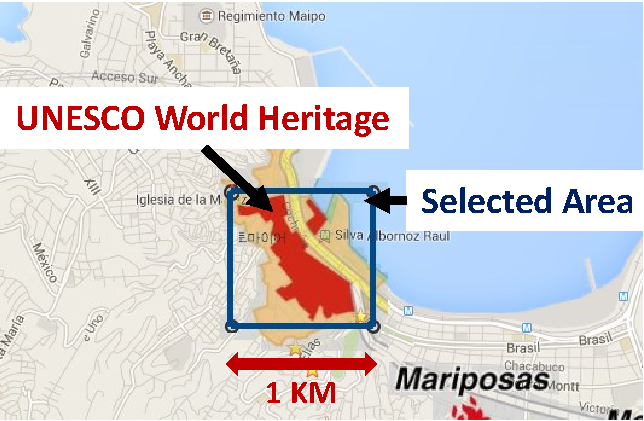
\includegraphics[scale=0.64]{figs/crawled_area}
	\vspace{-0.1in}
	\ourcaption{Selected sqare Km of Valparaiso
	including UNESCO World Heritage area.}
	\vspace{-0.1in}
	\label{fig:crawled_area}
\end{figure}

We choose Valparaiso, Chile as an target city to evaluate \name{}.
As shown in Figure~\ref{fig:crawled_area}, some area of Valparaiso is selected as UNESCO World Heritage because of its street arts.
Generated DB from street view images of carefully selected one square Km area including the world heritage.
We have done some experiments to prove that \name{} speeds up image searching and finally lower the searching cost enough to serve the service on web.

\oursubsection{Generating DB}
Google Maps provides an API to download street view images.
Allowed maximum field of view, FOV, is 120 degree so three images are needed to retrieve single stationary point.
We downloaded 30,000 street view images with Google Maps APIs and removed duplicants to obtain 12,129 unique street view images.
Then we SURFed each image and generated DB file.
The DB file was 1.2 GB large and consists of 4.4 million feature vectors.

\begin{figure}[t]
	\centering
	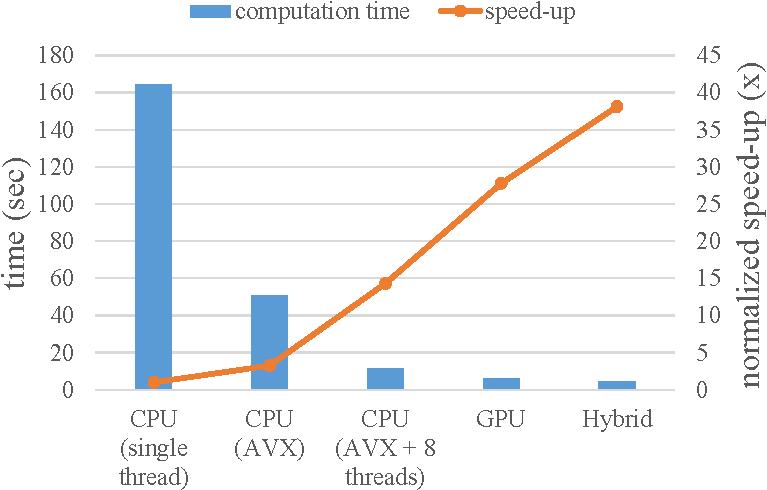
\includegraphics[scale=0.64]{figs/speed_up}
	\vspace{-0.1in}
	\ourcaption{Speed up of vactor matcing
	by each design choice or optimization.}
	\vspace{-0.1in}
	\label{fig:speed_up}
\end{figure}

\oursubsection{Searching Speed}
We built five versions of \name{} to compare contributions to searching speed of each design decision or implmentation.
We downloaded an image whose size is 859x1276 by web searching from Google with search key word of "Valparaiso street art".
We put that image to \name{} as an input and measured the time consumed by vector matching.
Figure~\ref{fig:speed_up} shows the result.
\name{} found the exact location where the street art exists.
We can observe that AVX optimization speeds up performance of single CPU core 3.25 times.
This is smaller than we expected (8 times) because an AVX instructions cannot be done in single cycle of CPU while normal floating point calculation can.
Another interesting observation is that GPU searching is two times faster than multi-threaded and AVX-optimized CPU search.
Lastly, a hybrid search, which uses both CPU and GPU, achieves 38 times faster speed than single-threaded search (165 seconds to 4.3 seconds).

%\oursubsection{Correctness}
